\clearpage
\paragraph{GPS}
For finding out the current position, speed and time of day a \verb|GPS| unit is used.

The unit connects as a serial USB device. There are two possible baudrates that can be
selected at compile time using \verb|C preprocessor directives|.

\begin{figure}[!htb]
    \centering
    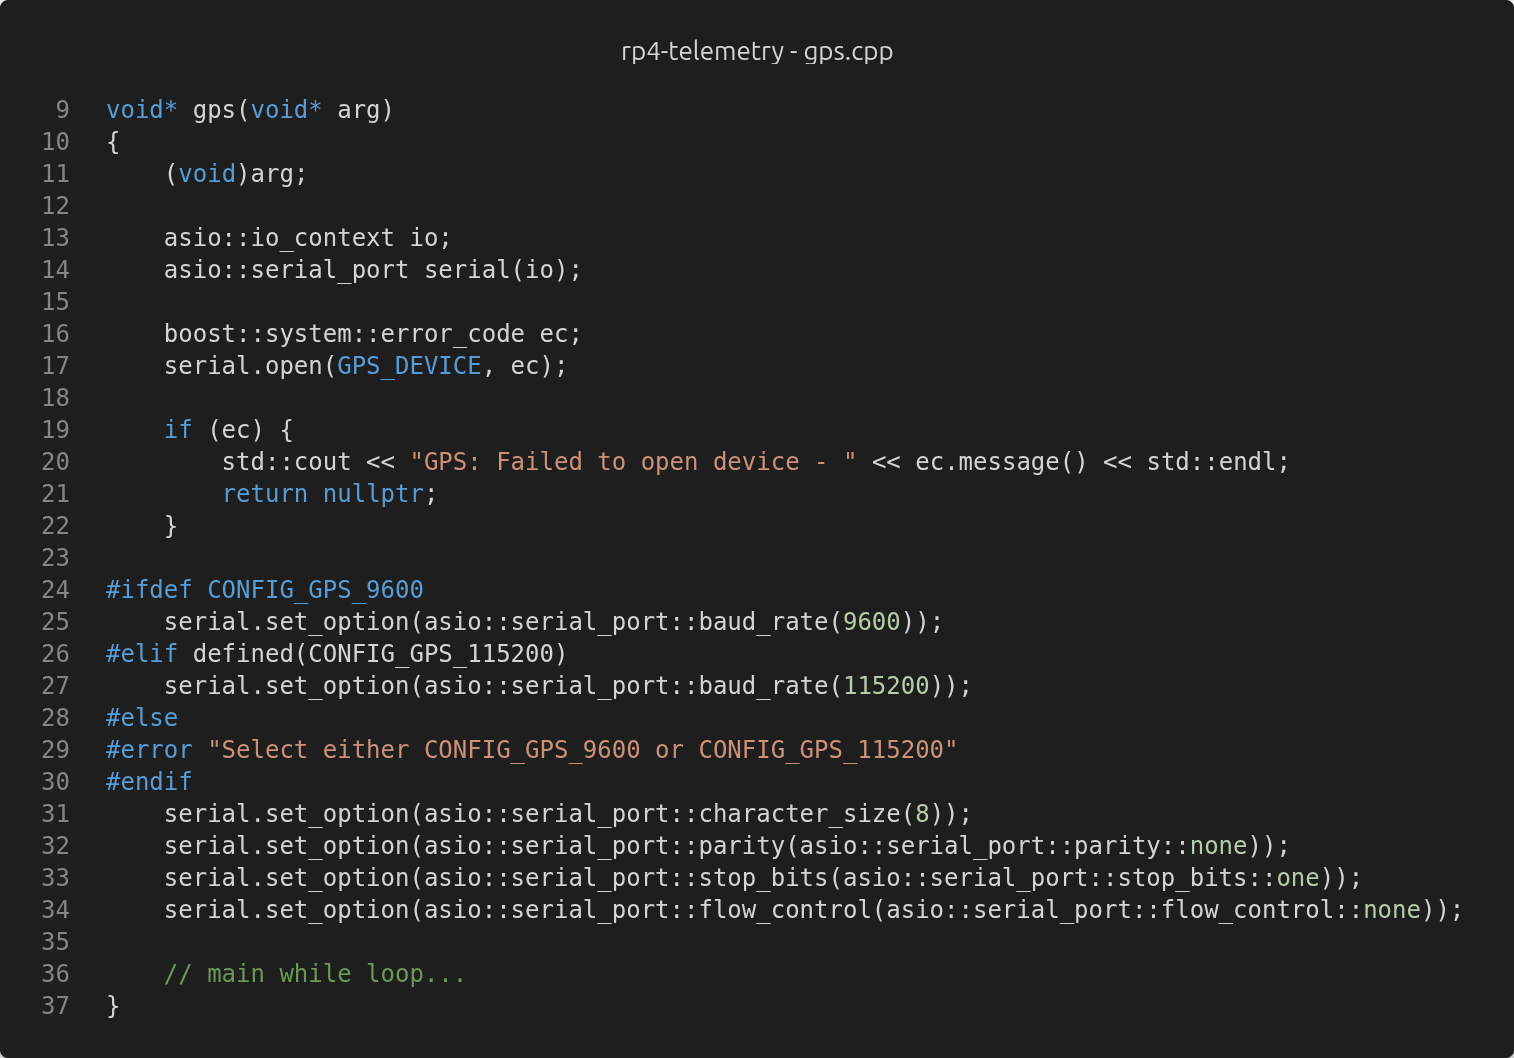
\includegraphics[width=\textwidth]{images/code/gps_setup.png}\par
    \caption{Setting up the GPS serial device}
    \label{fig:code-gps-setup}
\end{figure}
\FloatBarrier

The obtained information is in the form of \verb|NMEA 0183| packets.
These packets are then parsed using a library called \verb|minmea|.

The \verb|NMEA| standard defines several types of sentences,
that are used to specify which type of information is being transported.

The sentences that are of interest to the telemetry are:
\begin{itemize}
    \item GGA --- Global Position System Fix Data
    \item GLL --- Geographic Latitude and Longitude
    \item GSV --- GNSS Satellites in View
    \item RMC --- Recommended Minimum Specific GNSS data
    \item VTG --- Track made good and speed over ground
    \item ZDA --- Time and Date
\end{itemize}

Only the most important of these are shown in the code listing due to space constrains.

\begin{figure}[!htb]
    \centering
    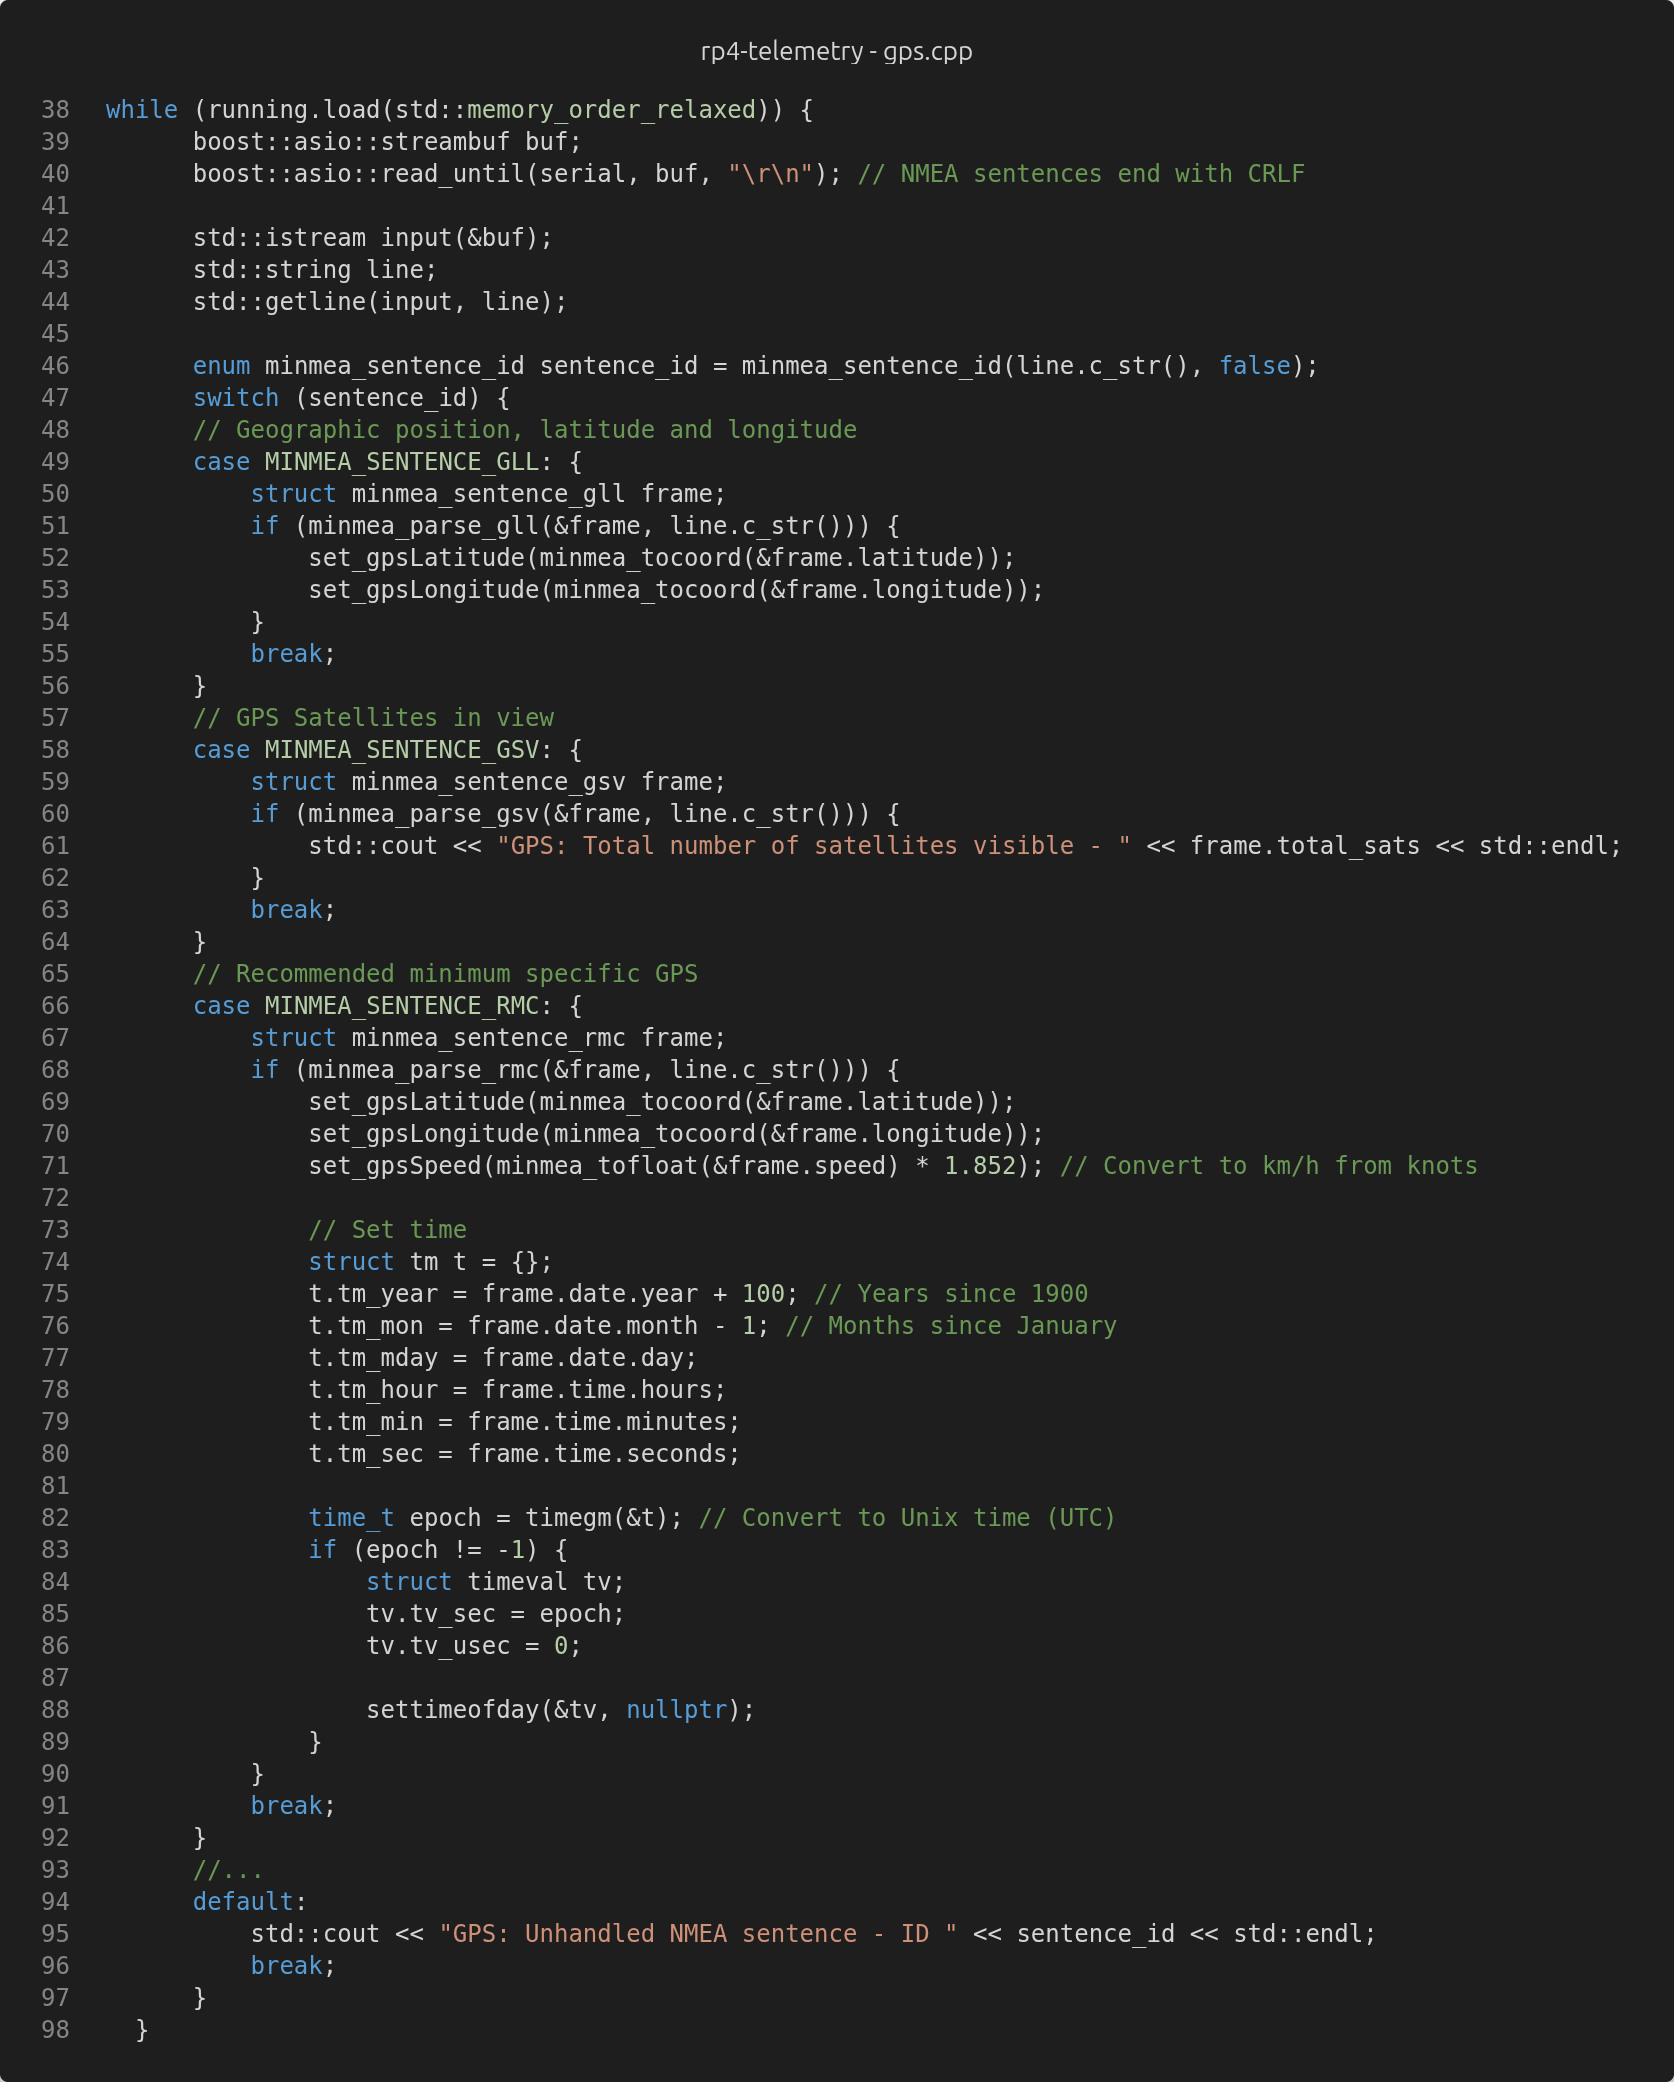
\includegraphics[width=\textwidth]{images/code/gps_read.png}\par
    \caption{Reading the GPS NMEA packets}
    \label{fig:code-gps-read}
\end{figure}
\FloatBarrier

% TODO go into detail about the sentence types
% TODO write more about what's on the screenshots